\section{Experimental Results}
\label{sec:result}

This section presents experiment results and answer the RQs by
studying the results quantatively and qualitatively.

\InputWithSpace{tables/manual-study-table}
\InputWithSpace{tables/test-results-table}

\subsection{RQ1: \tool Sentiment Label Consistency}
Table~\ref{table:ManualStudy} shows the statistics of scores collected
from the manual study of \tool. First column represents type of test
case. The number of test cases used for the study is represented in
second column. Label consistency score and \lc relevancy score defined
at equation~\ref{metric:srel} and~\ref{metric:lcrel} are shown at the
remaining columns. First, it is shown that high label consistency
score over 0.8. It means that \tool generates test oracles consistent
to human understanding. It is also observed that there is no
difference of the scores between seed and expanded sentences. The
observation implies that the expansion method in \tool preserves
sentiment of expanded sentences as its seed, and provides its
reliability. These observations answer RQ1 and conclude that \tool
generates test case with high consistency between test sentence and
its oracle.

\subsection{RQ2: Correctness of Linguistic Capability Categorization}
The result in table~\ref{table:ManualStudy} also shows that \tool
achieves high order of agreement with human assessment on \lc
relevancy. In parallel, it is observed that the expanded sentences
generated from \tool also have same level of \lc
relevancy. Accordingly, we answer the RQ2 by concluding that
\tool generates \lc relevant test cases with the agreement with human.

\jl{The following needs to be in RQ2 result section after simin
  completes RQ2 result section} Table~\ref{table:TestResult} shows
results of evaluation of three \sa models. First column lists
linguistic capability for \sa task, and Columns 2-3 show the number of
seed and expanded test cases respectively. Columns 4-5 show the
failure rate in percentage by running the \sa models on the seed and
expanded test cases respectively. Column 6 shows the number of
expanded test cases failed, but their seed test cases passed. For LC9,
we combine two 

From the
table, we can observe that 

\subsection{RQ3: Test Suite Diversity}

\begin{figure}
    \centering
    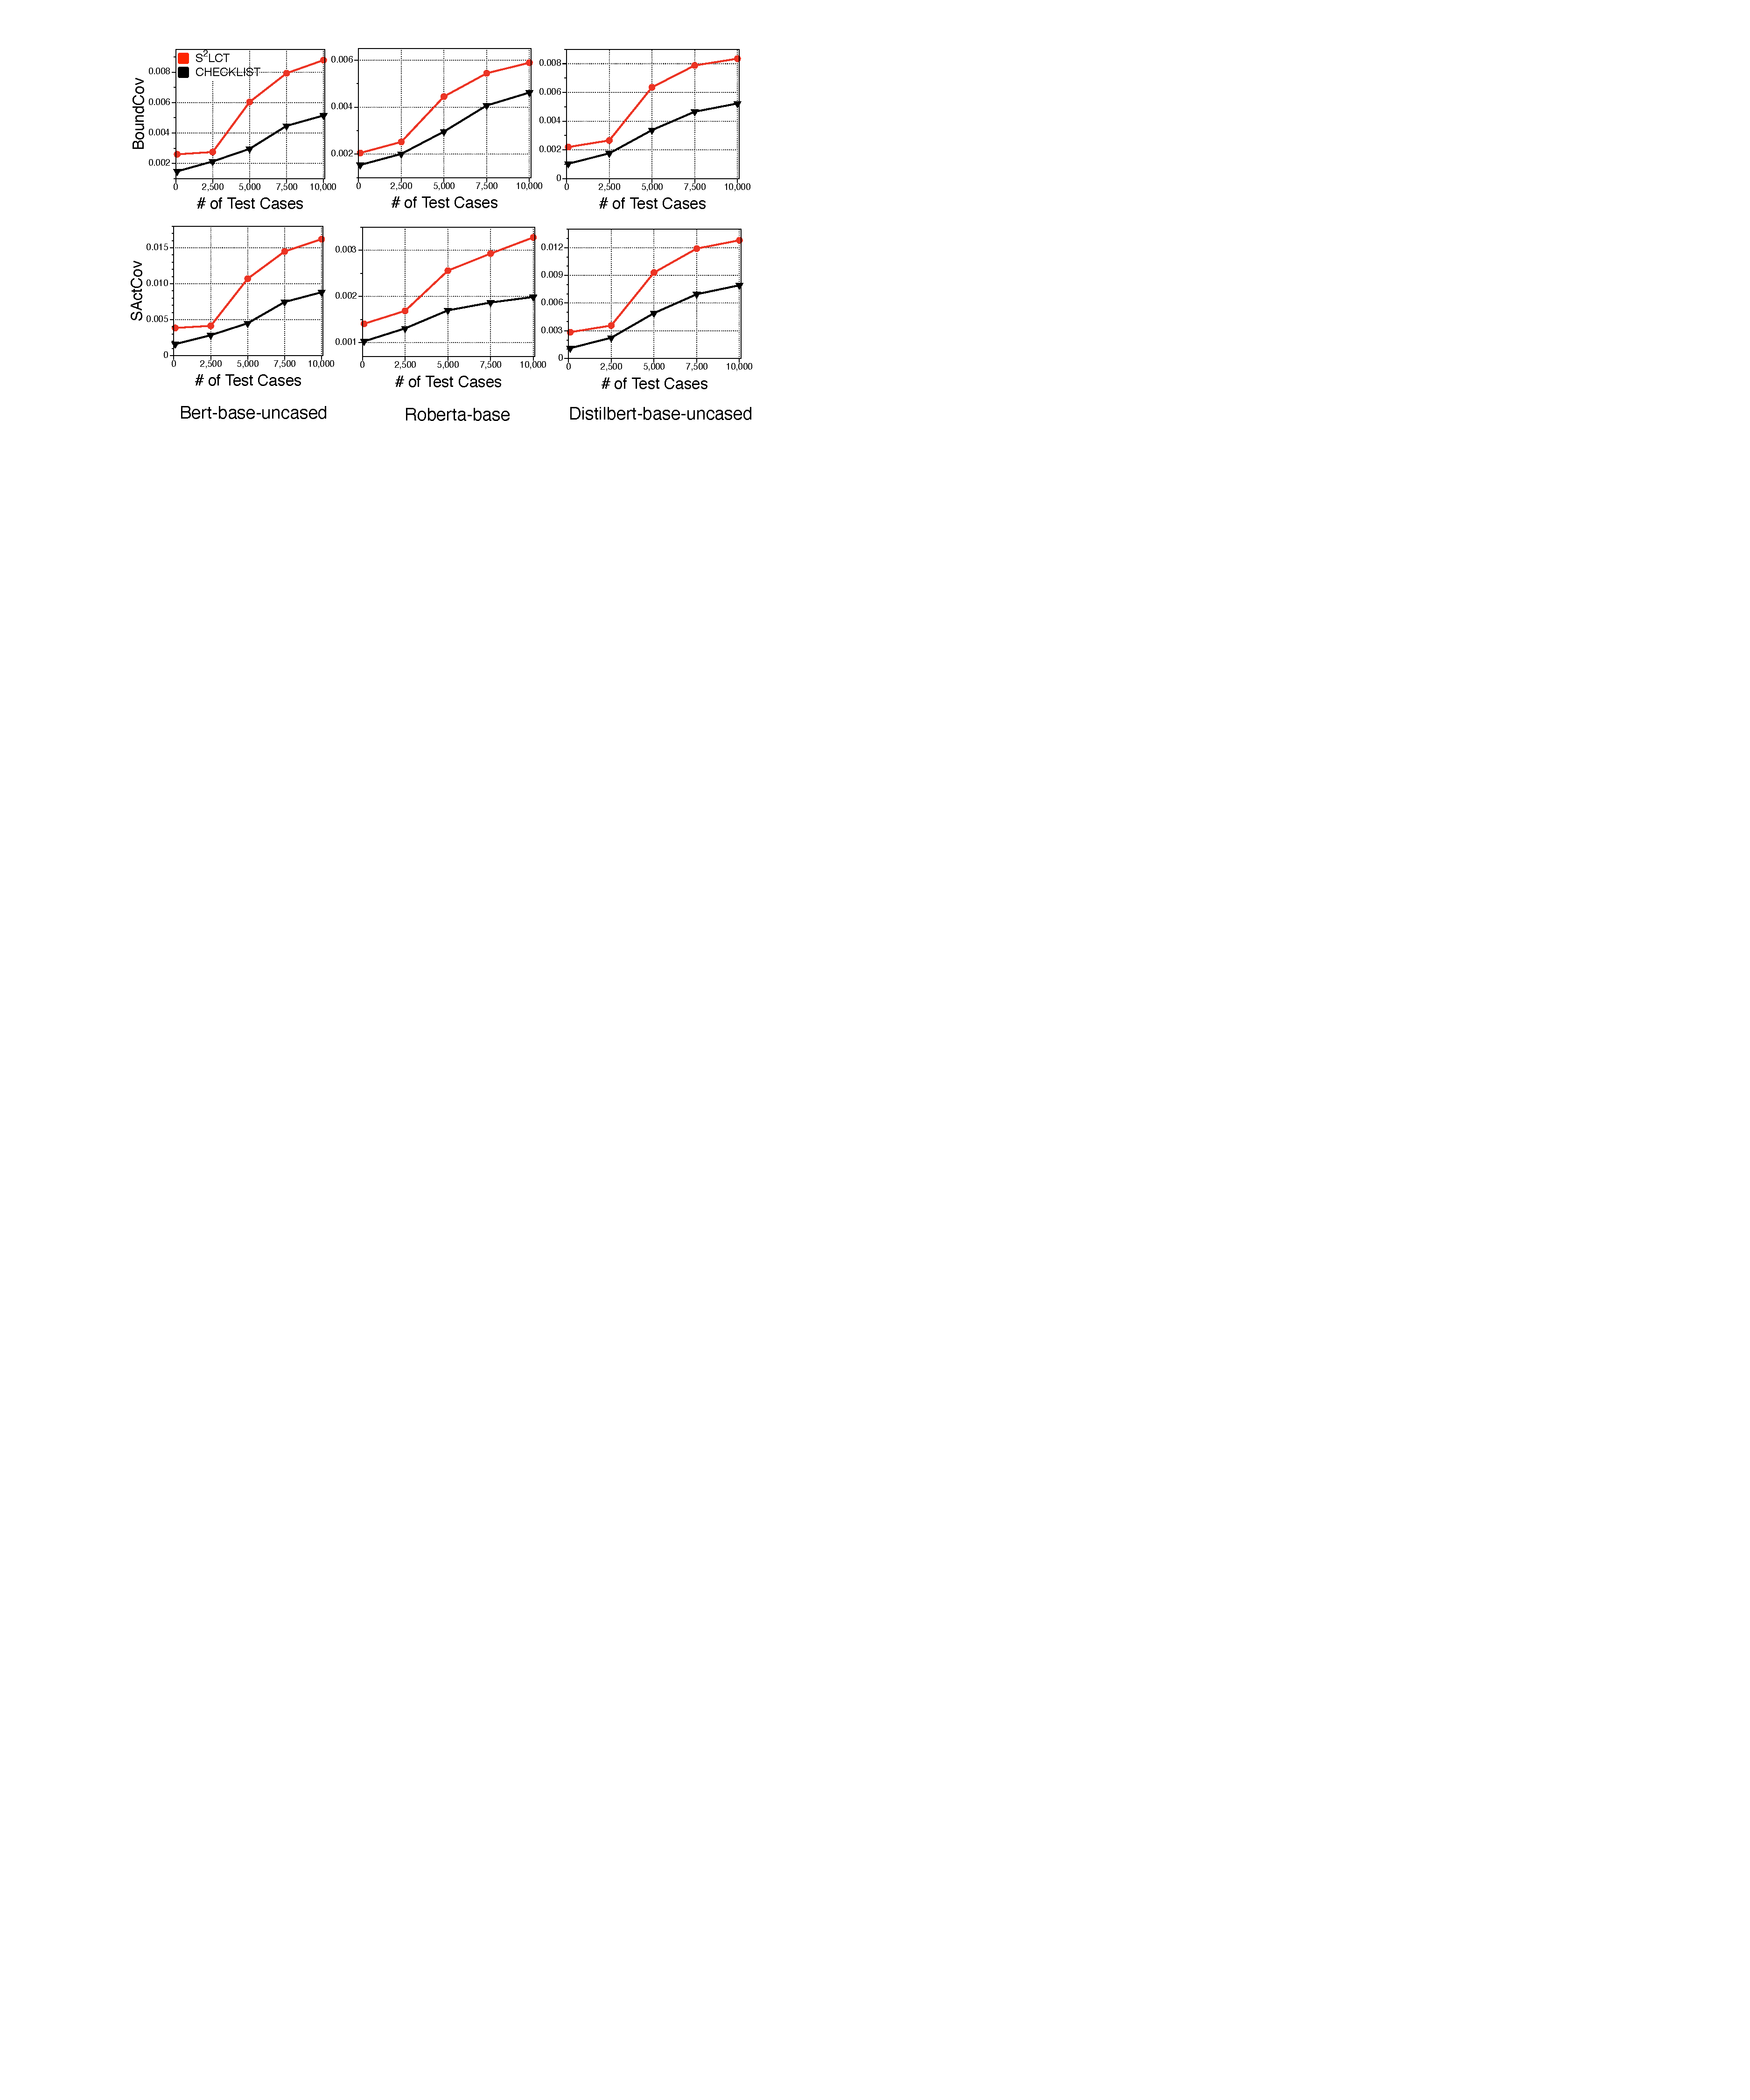
\includegraphics[width=0.5\textwidth]{figs/coverage.pdf}
    \vspace{-4mm}
    \caption{Coverage results of \tool and \Cklst test cases.}
    \label{fig:coverage}
\end{figure}

Next, Figure \ref{fig:coverage} shows the coverage results of \tool and \Cklst test cases. The red line represents \tool coverage and the black line represents \Cklst coverage. Each column in Figure \ref{fig:coverage} represents the results for one NLP model. The first row is the \textit{BoundCov} results and the second row is the \textit{SActCov} results.

We made three observations.
First, for \emph{all} experimental settings (i.e., NLP model and coverage metric), \tool achieves higher coverage than \Cklst. Recall that a higher coverage implies the test cases are more diverse and do not have a similar statistical distribution to the model training data. As a result, a test suite with greater coverage complements the model training data distribution (\ie holdout testing data) better.
For example, for the first NLP model under test, \tool can achieve a higher coverage than \Cklst with only half the number of test cases.
This result confirms that \tool can generate more diverse test cases to complement the holdout dataset for testing NLP models.

Second, as the number of test cases increases, the test suite can achieve better coverage. Such observation is intuitive. However, generating a more extensive test suite is not easy, particularly  for \Cklst, which is a manually template-based approach.

Third, for each NLP model, there is no fixed relationship between \textit{BoundCov} and \textit{SActCov}. In other words, while a test suite may produce higher \textit{BoundCov} for some models, the same test suite may get higher \textit{SActCov} for other NLP models.
Recall that \textit{BoundCov} measures both the upper and lower corner neurons and \textit{SActCov} measures only the upper corner neurons. 
Such observation implies that the upper and lower corner neurons are distributed unevenly, and measuring only one of them is not enough.

\subsection{RQ4: Use \tool for Debugging}
